\documentclass[11pt,a4paper]{article}
\usepackage{amsmath}
\usepackage{mathtools}
\usepackage{graphicx}
\graphicspath{ {/home/alisa/uni-sven/proj/pics/} }

\begin{document}
\title{Development and programming of a micro processor}
\author{Alisa Dammer and Sven-Hendrik Haase}
\maketitle

\section{Introduction}
\subsection{General information: How does CPU work}
A central processing unit (CPU) is a heart of a computer. It presents arithmnetical logic, logic operations and input-output operations. Nowadays one computer can have more than one CPU, called multiprocessors. But in this project we have concentrated our attention on one single microprocessor.\\
In order to work properly and execute commands (perform certain operations), CPU needs to go through several stages:
\begin{enumerate}
	\item[1.] Fetch: read the program, that is stored in memory as instructions. (We implemented an Assambeler, that translates the program from "human" language to instructions. More about it in  section "CPU implementation"). To keep an eye on right order of instructions Program Counter (PC) keeps the address of the next executable instruction.
	\item[2.] Decode: Instruction is a representation of a assembly command in 0 and 1. During this stage every executable instruction is broken up into several parts. The amount and length of these pieces depend on the type of instruction (more details in the next section). 
	\item[3.] Execute: According to what kind of instruction has to be performed, different units of the CPU can be involved. For example: ALU and two registers, or CU and register etc. Normally modern CPUs have overflow flags, that are "activated", if the output is too big for restricted CPU (by "restricted" we mean, that all CPUs are by design implemented to deal with limited values).
	\item[4.] Writeback: During this stage the result of an instruction is "returned" to some memory part, so that it could be used later on.
\end{enumerate}

All these 4 steps repeat for every instruction until the "stop" instruction is reached (logical end of the program), which is normally refers to "no action" or "terminate". As was mentioned above in Fetch-stage, PC holds the address of the next executable instruction, incrementing each time the instruction is executed. Some of control instructions like "jump" change PC according to needs of the program, for example by implementing a cycle.\\
\subsection{Main components of a simple CPU}
Every CPU's design starts with Instruction Set Architecture (ISA) definition, that describes what particular prozessor is capable of: general specification (word length, instruction length), instruction specifications and opcodes (operations, that can be presented in binary form), type of memory that is used (number of special purpose and general purpose registers), and other specific infromation if needed. \\
Apart from ISA all microprozessors have certain units like: Program Counter (PC), Control Unit (CU), Aruthmetic Logic Unit (ALU), Registers (Register Bank), Buses.\\
\begin{center}
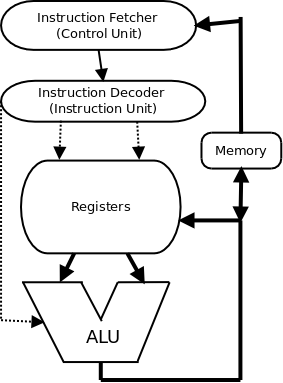
\includegraphics[scale=0.5]{simpleCPU3.png}
\end{center}

However our implementation differs from existing ones. This will be shown in details in next section.\\ 

\newpage
\section{CPU implementation}
\subsection{Instruction Set Architecture}
As was mentioned in the previous section, ISA defines all specifications of a CPU. In our work we decided to stop on 16bit instructions, that have the same lenght as word, so we didn't have to think about instructions consisting of more than one word, which also makes Instruction Unit (our "instruction breaker") easier to implement.
\begin{verbatim}
general specifications:
	16 bit instructions
	16 bit words
	14 registers:
		8 general purpose registers
		6 special purpose registers
\end{verbatim}
Our cpu has only one type of instructions, also we don't have special flags. Instead of special flags we use special purpose registers and certain instructions. As already was said: we have implemented pretty simple microprocessor.
\begin{center}
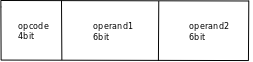
\includegraphics[scale=0.7]{instruction1.png}
\end{center}
Because we have set the lenght of opcode to 4 bits, we could have only 16 = 2²(to the power of 2) But we have 16 opcodes for "real" instructions and 18 "pseudo" instructions without opcode, but they are replaced with composition of actual instructions. For example, instruction "add" opeartes with two registers, saving result of the operation to the left (or first) register:
\begin{verbatim}
movi a 5
movi b 4
add a b
stop
\end{verbatim}
This program will result in:
\begin{verbatim}
program start
PC0 => movi a 7
PC1 => movi b 4
PC2 => add a b
program end
--------------------
registers:
zero: 0
pc: 3
cmp_result: 0
jmp_next: 0
tmp1: 0
tmp2: 0
a: 11
b: 4
c: 0
d: 0
e: 0
f: 0
g: 0
h: 0
\end{verbatim}
Here as first example all registers, that we have are shown, later on only registers, that get some value will be shown. "Program end" - is our "stop" instruction (Mostly known as HALT). So the result is that register a gets the value 11 = 7 + 4. We didn't implement any special output register, cause we can always store (or move to desirable "output"-register) data manually.\\
Both only actual instruction list and all-instruction list can be found in our isa.txt file.\\
Pseudo instructions can be represented by composition of actual instructions. Some of them consist of two instructions, some of them contain up to 5 instructions. For example:
\begin{verbatim}
movi a 7
addi a 5
stop
\end{verbatim}
The original program consist of 3 instructions, but it results in program with 4, because addi is a pseudo instruction replaced with movi and add instructions.
\begin{verbatim}
program start
PC0 => movi a 7
PC1 => movi tmp1 5
PC2 => add a tmp1
program end
--------------------
\end{verbatim}
Another example for a pseudo instruction would be "modulo" program, 45 mod 10 = 5
\begin{verbatim}
movi a 45
movi b 9
mod a b
stop
\end{verbatim}
But it will result in:
\begin{verbatim}
program start
PC0 => movi a 45
PC1 => movi b 10
PC2 => mov tmp1 a
PC3 => div a b
PC4 => mul a b
PC5 => sub tmp1 a
PC6 => mov a tmp1
program end
--------------------
registers:
pc: 7
tmp1: 5
a: 5
b: 10
\end{verbatim}
Apart from instructions (opcodes) and general information ISA gives information about REGISTERS: general and special purpose.
\begin{verbatim}
registers:
	zero 		000000 # always returns value 0
	
	pc			000001 # program counter
	cmp_result  000010 # result of comparison as defined below
	jmp_next    000011 # je will go here if the comparison succeeds
	tmp1        000100 # temporary register to be used by compiler
	tmp2		000101 # another temporary register

	# general purpose registers
	a       	000110
	b       	000111
	c      	 	001000
	d       	001001
	e       	001010
	f       	001011
	g      	 	001100
	h       	001101
\end{verbatim}
In our project we decided not to implement both ALU and CU, but unite them in control Unit. Execution of a programm in our cese goes through following stages:
\begin{enumerate}
	\item[1.] Encode - assembly programm is "translated" with the help of written Assembler to binary string. Outout file gets an extention ".o" and consist of N 16bit strings, where N is a number of "actual instructions" (here, if pseudo instruction is used in the programm, it is translated into several actual instructions for further executing). So, as the resukt we get Machine Code.
	\item[2.] Decode - every instruction in output file is split into 3 parts: opcode, operand 1 and ooperand 2 according to number of bits specified in ISA. So, as the result of this stage we get executable instructions, where we know what operations with what operands should be performed. 
	\item[3.] Execution - actual performing of operations with given values, using memory and registers according to the originally written .asm programm. As the result of executing a program we get the result "stored" in desirable memory location or register (if specified in the program), or by default in the last "mentioned" left register.\\
Our CPU can be presented as following schema:
\end{enumerate} 
\begin{center}
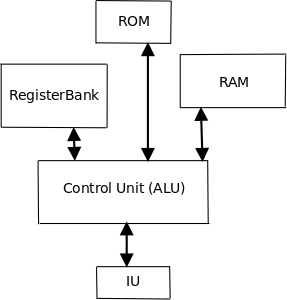
\includegraphics[scale=0.7]{ourCPU.png}
\end{center}

\newpage
\subsection{Assembler}
As was told earlier, our first stage of the program execution is encoding of the program for futher use. This happens in assempler.py unit in following order:
\begin{enumerate}
	\item[1.] First, the input file with .asm extention is opend into source file for reading, splited into root and extenion. And binary file is created with extention .o.
	\item[2.] This binary file for every code line	"translates" human code into bit-string, that machine can interprete.
	\item[3.] Depending on type of instruction, whether it is an actual or pseudo instruction command will be converted into 1 or more bit-strings. (examples of pseudo instructions are given above). Every bit-string is added to the binary file. As the result we get a list containing N bit-strings.
\end{enumerate}
For example with modulus binary file will look like this:
\begin{verbatim}
alisa@comrade ~/u/proj> python2 assembler.py programs/test.asm
['0100000110101101', '0100000111001001', '0011000100000110',
 '1000000110000111', '0111000110000111', '0110000100000110',
 '0011000110000100', '0000000000000000']
\end{verbatim} 
Assembler contains "translating rules" for all instructions mentioned in ISA, so that Control Unit (in our case also ALU) deals only with actual opcodes and executes only them.\\

\subsection{Memory and Registers}
Every Prozessor has a memory unit - physical device for working with the program. There are two memory types existing: non-volatile (flash memory,  ROM/PROM/EPROM/EEPROM) and volatile (RAM, DRAM).\\
Non-volatile memory is normally used for storing information for long-term use without its change (overwritting is possible, but it requires much more time and thus not efficient for temporary and "local" computations).\\
In our Implementation ROM gives "the number of certain actual instruction" back - holds the address of the instructions. ROM is initialized inside simulation program as well as Control Unit. In code realization ROM has 3 parameters: Rom(dout, addr, CONTENT), where first two are pretty clear. The third parameter of ROM is initialized with the help of special function "load\_program(path)", that loads the program into list of instructions and returns teh list of instructions as unsigned shorts. Afterwards every decoded instruction is assigned an  unique integer, which represents certain location (adrress) in static memory.\\
Currently most commonly used types of a volatile memory (RAM) are static RAM (SRAM) and dynamic RAM (DRAM). But it is mostly hardware (production difference), since we have a simulation only, we didn't have to work with specific memory type. In this project RAM is limited with 32 memory-cells. Both RAM and ROM can hold value up to 2(to the power of 16). \\
In implementation of this project we have only one channel.git Single-channeling is mostly the result of our wrong descision made in the ver beginning: we decided to implement a register bank along with memory, but we used the naive realization - a list of registers. We could built distinct registers inside of control unit, so that we had access to separate registers without any time dependency (here the dependency between registers at one clk.posedge is meant).\\
Apart from non- and volatile memory we have implemented Register Bank, that consists of 14 registers splited into two groups: general purpose and special purpose registers.\\
Since our CPU is quite limited, we don't need many registers to work with. We have implemented special registers to partially substitute flags and some hardware units. For example we have "pc" register, that gets the adress of next instruction directly from CU (we don't have selfseficient Program Counter, in our case the number of next instruction is the number of the line, where particular instruction is located).\\

\subsection{Instruction Unit}
Since we have restricted the lenght of words and instruction size to the same value (16bit, or 2byte), decoding an instruction became really easy:
according to in ISA specified instruction type opcode gets first 4bit, than operand1 gets next 6 bit and the last 6bit gets operand2. Some opcodes require only one operand ("not"). It is implemented so, that if you type in second operand, it is won't influence the result, because by the implementation second operand is ignored.
for example:
\begin{verbatim}
movi a 3
movi b 9
not a b
stop
\end{verbatim}
Will result in:
\begin{verbatim}
program start
PC0 => movi a 45
PC1 => movi b 9
PC2 => not a
program end
--------------------
registers:
zero: 0
pc: 3
cmp_result: 0
jmp_next: 0
tmp1: 0
tmp2: 0
a: 65533
b: 9
\end{verbatim}
As you can see, the second operand is really ignored.\\

\newpage
\subsection{Control Unit}
Classically, CU handle the operation of the whole prozessor, it manages communication between in- and output devices, interprets and executes them itself, or via ALU. Also, Control Unit provides control signals, like clock (clk in our code). CU performs all four stages of executing a program.\\
In our project the Control Unit is implemented inside of cpu-simulation, and the instances of RAM, ROM; Register Bank and Instruction Unit are controlled by CU but as separate units. This leads to some inefficiency, like singlethreading: one register at a time can be used. Program Counter, normally selfseficient unit implemented outside the CU, in our case is also build-in in the Control Unit. Since we have a special register for address of the next instruction, CU depending on two cases changes the value in pc-register. These two cases are:
\begin{enumerate}
	\item[1.] The instruction is already executed, and certain operations are successfully performed. Afterwards the value in pc-register is just incremeted (in "Memory and Registers" section it was shown how pc tracks the executable insruction and how does ROM is initialized). 
	\item[2.] The second possibility to chanhe the PC is by using flow control instruction. These are jump-opcodes. Here in special-purpose register "jmp\_next" the location of the jump (the adress of the next desirable instruction) is stored. If it conditions of the jump-operation match the result, than pc gets the value from "jmp\_next" register. This way cycles are normally implemented in assembly.	
\end{enumerate} 
So the way our CPU works is following:
\begin{enumerate}
	\item[1.] The program, written in Assembly is encoded by assembler.py (concerete examples and explanations are in "assembler" subsection).
	\item[2.] In the module "simulation.py" firts the programm is decoded with function "load\_program(path)"; the result is used as the third parameter for ROM initialization (all instructions in the program get their unique id for futher pc addressing). Also RAM, RegisterBank, Clock and Instruction Unit are initialized for futher operation of the Control Unit.
	\item[3.] In CU for every instruction opcode is defined and the proper action is performed with operands given in the instruction until opcode "stop" (0000) is reached. All nessussary output is printed.  
\end{enumerate}

\newpage
\section{Results}
\subsection{Test of the CPU}

\end{document}

